\documentclass{article}
\usepackage{macro}
\usepackage{graphicx}
\graphicspath{ {./} }
\title{Policy Gradient Methods for Deep Reinforcement Learning}
\author{Hongshan Li}
\begin{document}
\maketitle

RL is big and rich, its history traces back to Pavlov's study on the 
psychology of animal learning (conditional response) back in 1902.
The expository article History of Reinforcement Learning (http://incompleteideas.net/book/first/ebook/node12.html) is a good resource to learn
how RL evolved in the last 100 years.

Policy Gradient Methods is a class of RL algorithms that directly 
learns a policy from interaction with the environment. In contrast,
to this, one can also learn a state value estimate of the current
state of the env and the candidate actions. This class of algorithms
is called Q-learning. 


\textbf{Review about setups in RL}
The objective of RL is to find a policy $\pi$ that gets the highest 
rewards from a \emph{Markov Decision Process}

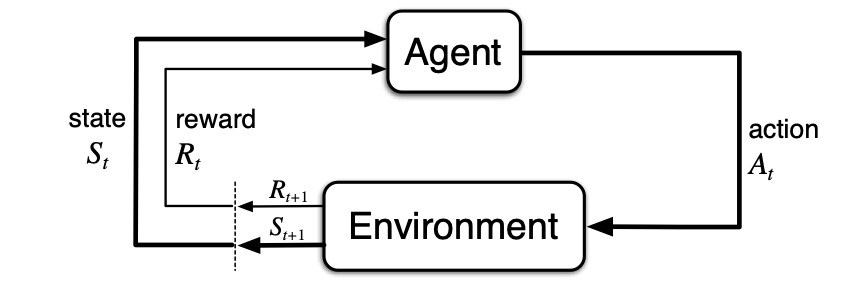
\includegraphics[width=8cm]{mdp}

A fundamental difference supervised learning and RL is that data is 
completely determined before any training, whereas in RL data is
dynamically generated through interaction with the environment. 
This means the distribution of the data for SL is static and the 
distribution of data for RL changes as the agent learns. 


\textbf{REINFOCE}



% \biblio
History of Reinforcement Learning
http://incompleteideas.net/book/first/ebook/node12.html
\end{document}

